\section{可以直接改的 LaTeX 示例}
下面的公式、表格、图片和参考文献都来自这个项目。你可以选择对应源代码，让 AI 解释语法，或在预览确认后修改。

\subsection{公式与交叉引用}
文字中的公式可以这样写：$E=mc^2$。需要编号的公式可以使用 \texttt{equation} 环境：
\begin{equation}
\label{eq:weighted-score}
S = \sum_{i=1}^{n} w_i x_i, \qquad \sum_{i=1}^{n} w_i = 1.
\end{equation}
式~\ref{eq:weighted-score} 是一个加权求和示例。这里的符号只用于语法练习，不代表一项真实研究的分析结果。

\subsection{一个简单的表格}
\begin{table}[htbp]
\centering
\caption{写作练习的三个步骤}
\label{tab:writing-steps}
\begin{tabular}{lll}
\toprule
步骤 & 你要做的事 & 可以向 AI 提的要求 \\
\midrule
起草 & 写出核心观点 & 帮我检查论点是否清楚 \\
推敲 & 核对结构与证据 & 指出缺少依据的地方 \\
定稿 & 统一术语与格式 & 润色选区，保留引用和命令 \\
\bottomrule
\end{tabular}
\end{table}
表~\ref{tab:writing-steps} 使用 \texttt{booktabs} 绘制横线。要增加一行，复制一行内容并修改即可。

\subsection{图片与图注}
\begin{figure}[htbp]
\centering
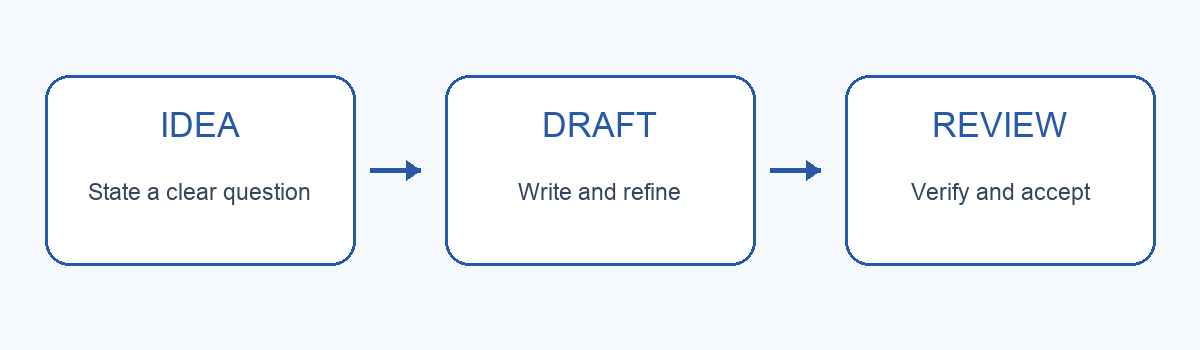
\includegraphics[width=0.93\linewidth]{figures/workflow.png}
\caption{先表达，再推敲，最后确认：人机共写的一个简单循环。}
\label{fig:writing-workflow}
\end{figure}
图~\ref{fig:writing-workflow} 使用项目中的 PNG 图片。可以询问支持视觉的模型：“读取这张图，帮我写一个更准确的中文图注。” 上传自己的图片时，尽量使用简单的英文文件名，并修改 \texttt{includegraphics} 中的路径。

\subsection{参考文献的最小示例}
\texttt{references.bib} 包含一个\textbf{明确标注为教学占位的条目}，可用命令 \verb|\cite{welcome-demo}| 引用，例如这里~\cite{welcome-demo}。项目编译时会生成文末的参考文献列表。

正式写作时，请用你已经核验过的真实文献替换占位条目，并同步更新引用键。不要把教程条目当作真实研究来源。

\section{现在，换成你的主题}
你可以保留这套文件结构，把标题改成自己的题目，再逐步替换正文。遇到编译错误时，先查看日志，定位文件和行号；向 AI 提问时，也可以粘贴相关错误信息，并让它先解释原因。

\begin{center}
\color{ScribeBlue}\large 让工具处理重复工作，把判断留给自己。
\end{center}
